\chapter{Digital Signal Processor}

%----------------------------------------------------------------------------------------
%	Section
%----------------------------------------------------------------------------------------

\section{ADSP-BF548 EZ-KIT Lite}

This section primarily summarizes the hardware-related information that helps developers write more robust and efficient C code.

%--------------------------------------------
%--------------------------------------------

\subsection{Hardware Architecture}

\textbf{Audio Codec} in charge of sampling speech and \textbf{Memory Hierarchy} that restricts the storage of variables are highly significant to the implementation on the DSP board.

%--------------------------------------------

\subsubsection{Audio Codec}
An Analog Devices AD1980 audio codec is the audio interface of the EZ-KIT Lite. The codec connects to multiple audio connectors (3.5 mm) which allow us to get audio in and out. These connectors can be easily found at the bottom left corner of the board.

\begin{figure}[H]
\centering
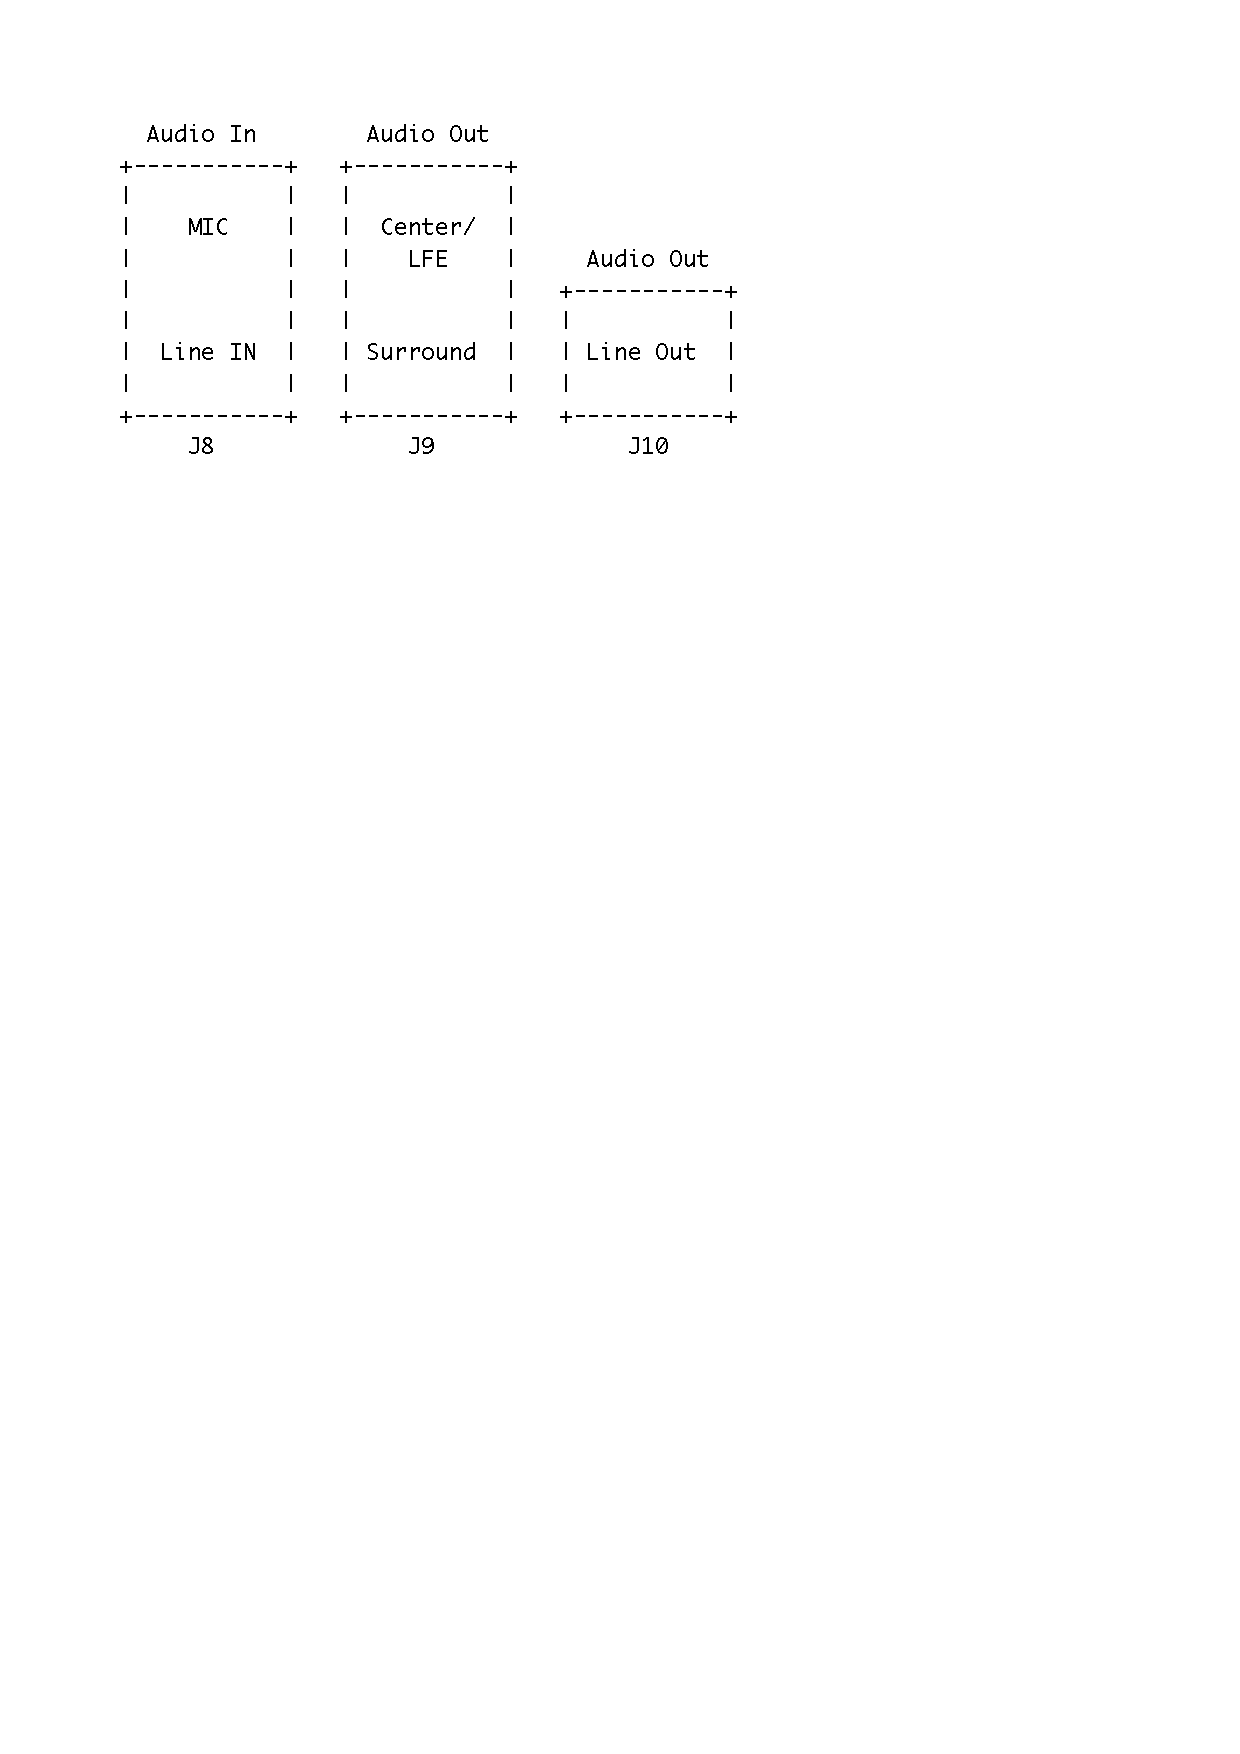
\includegraphics[width=3in]{ang/audio-connectors}
\caption{Audio Connectors}
\label{audio-connectors}
\end{figure}

Fig. \ref{audio-connectors} illustrates that the top location of \texttt{J8} is for a stereo microphone and the bottom location is for a stereo line in. According to Fig. \ref{AD1980-schematic}, the difference between \texttt{MIC} and \texttt{LINE IN} is signals via \texttt{MIC} will be pre-amplified. The preamp gain is collaboratively controlled by \texttt{MIC} Volume Register (\texttt{AD1980\_REG\_MIC\_VOL\_CTRL}) and Miscellaneous Control Bit Register (\texttt{AD1980\_REG\_MIC\_VOL\_CTRL}) \cite{AC97-codec}. In addition, it can be clearly seen that AD1980 can only sample 2 channels at any given moment due to the RECORD SELECTOR multiplexer. Thus, we decide to input noisy command and noise via the left / right channel of \texttt{MIC} respectively.

\begin{figure}[H]
\centering
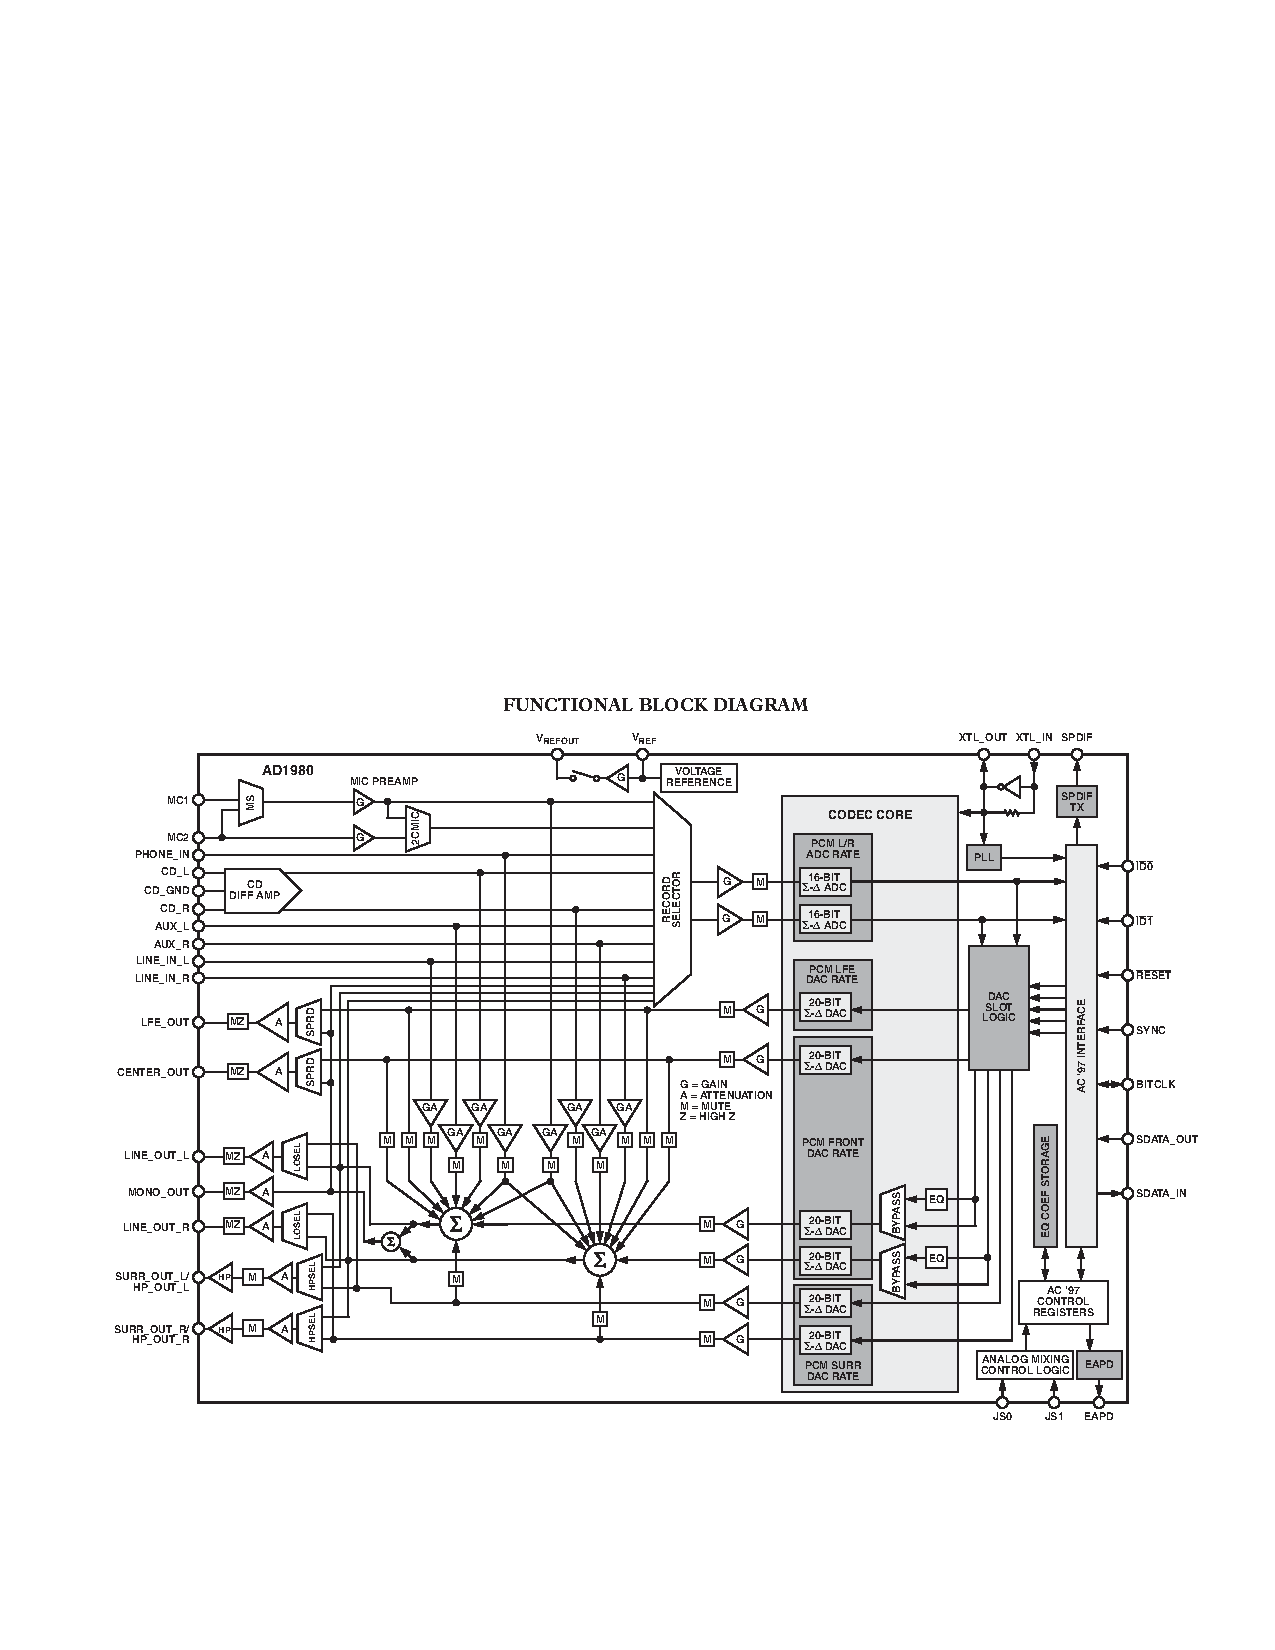
\includegraphics[width=6in]{ang/AD1980-schematic}
\caption{AD1980 Functional Block Diagram}
\label{AD1980-schematic}
\end{figure}

%--------------------------------------------

\subsubsection{Memory Hierarchy}
The ADSP-BF548 processor supports a hierarchy of three synchronous memories.\\

Internal L1 memory consists of two 32 KB data SRAM banks \cite{bf54x-hardware}. L1 memory is the highest-performing memory available to the Blackfin core and can be accessed at core clock speeds \cite{start-with-bf548}.\\

Internal L2 memory consists of a single 128 KB area of SRAM. L2 is slightly lower-performing than L1, requiring two core clock cycles for access. L2 provides more capacity accompanied by higher latency. \cite{start-with-bf548}\\

External memory is a 64 MB DDR SDRAM that exists external to the processor mounted on the DSP board. External memory operates synchronously with the system clock rather than the core clock, causing access time to SDRAM to be relatively slower than to L1 or L2 memory \cite{start-with-bf548}. 64 MB (67108864 bytes) is enormous given that each \texttt{float} / \texttt{fract32} variable occupies 4 bytes. Hence, we will pre-compute reusable coefficients as long as fetching them from external memory is faster than computing them. In fact, L1 \& L2 are big enough to store these coefficients, decisions will be elaborated in detail in the following \textit{C Program} section.

%--------------------------------------------
%--------------------------------------------

\subsection{Data Types}

\subsubsection{Directly Supported Data Types}

The compiler directly supports ten scalar data types as shown in Table \ref{fixed-point-data-types} and Table \ref{floating-point-data-types}. Note that \texttt{long} is equivalent to \texttt{int} and \texttt{double} is equivalent to \texttt{float}.

\begin{table}[H]
\centering
\begin{tabu} to \textwidth {XXXX}
\toprule
Type &Size &Min &Max\\
\hline
\texttt{char} &8-bit &-128 &127\\
\hline
\texttt{unsigned char} &8-bit &0 &255\\
\hline
\texttt{short} &16-bit &-32,768 &32,767\\
\hline
\texttt{unsigned short} &16-bit &0 &65,535\\
\hline
\texttt{int} &32-bit &-2,147,483,648 &2,147,483,647\\
\hline
\texttt{unsigned int} &32-bit &0 &4,294,967,295\\
\hline
\texttt{long} &32-bit &-2,147,483,648 &2,147,483,647\\
\hline
\texttt{unsigned long} &32-bit &0 &4,294,967,295\\
\bottomrule
\end{tabu}
\caption{Fixed-Point Data Types}
\label{fixed-point-data-types}
\end{table}

\begin{table}[H]
\centering
\begin{tabu} to \textwidth {XXX}
\toprule
Type &Size &Range\\
\hline
\texttt{float} &32-bit &$\pm 1.18 \times 10^{-38}$ to $\pm 3.4 \times 10^{38}$\\
\hline
\texttt{double} &32-bit &$\pm 1.18 \times 10^{-38}$ to $\pm 3.4 \times 10^{38}$\\
\bottomrule
\end{tabu}
\caption{Floating-Point Data Types}
\label{floating-point-data-types}
\end{table}

\begin{figure}[H]
\begin{minipage}[t]{0.5\linewidth}
\centering
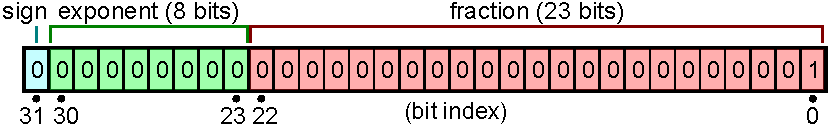
\includegraphics[width=\textwidth]{ang/smallest-denormalized-number}
\caption{Smallest Denormalized Number}
\label{ang/smallest-denormalized-number}
\end{minipage}
\begin{minipage}[t]{0.5\linewidth}
\centering
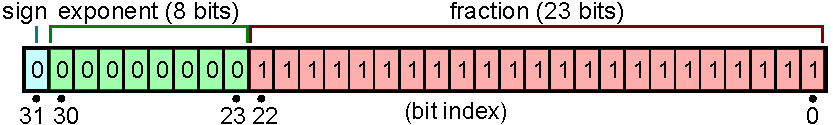
\includegraphics[width=\textwidth]{ang/largest-denormalized-number}
\caption{Largest Denormalized Number}
\label{ang/largest-denormalized-number}
\end{minipage}
\end{figure}

\begin{figure}[H]
\begin{minipage}[t]{0.5\linewidth}
\centering
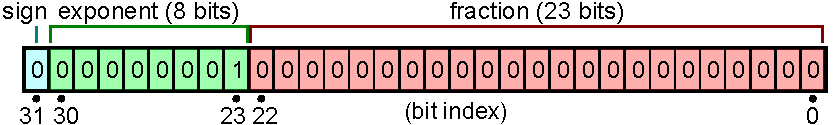
\includegraphics[width=\textwidth]{ang/smallest-normalized-number}
\caption{Smallest Normalized Number}
\label{ang/smallest-normalized-number}
\end{minipage}
\begin{minipage}[t]{0.5\linewidth}
\centering
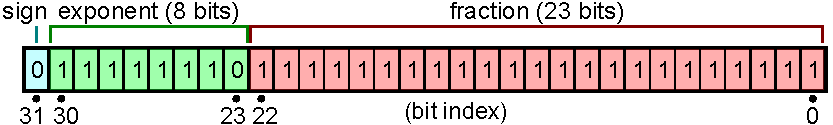
\includegraphics[width=\textwidth]{ang/largest-normalized-number}
\caption{Largest Normalized Number}
\label{ang/largest-normalized-number}
\end{minipage}
\end{figure}

Fig. \ref{ang/smallest-denormalized-number} to Fig. \ref{ang/largest-normalized-number} demonstrate the internal representation of a single precision floating-point number. The actual mantissa (fraction part) includes 23 fraction bits to the right of the binary point and an \textit{implicit leading bit} to the left of the binary point. When the exponent part is equal to $(00000000)_2$, the implicit leading bit is with value 0 (denormalized); otherwise, the implicit leading bit takes 1 (normalized). Hence, the total length of mantissa is $(23 + 1)$ bits; in other words, \texttt{float} has a precision of $\log_{10}(2^{24}) \approx 7.225$ decimal digits. This deduction is significant to exporting model and coefficients from MATLAB.

\begin{align}
value &=
\begin{cases}
(-1)^{b_{31}} \times (0.b_{22}b_{21} \dots b_{0})_2 \times 2^{- 126} &\text{denormalized}\\
(-1)^{b_{31}} \times (1.b_{22}b_{21} \dots b_{0})_2 \times 2^{(b_{30}b_{29} \dots b_{23})_2 - 127} &\text{normalized}
\end{cases}\\
&=
\begin{cases}
(-1)^{b_{31}} \times \sum_{i=1}^{23} b_{23-i} 2^{-i} \times 2^{- 126} &\text{denormalized}\\
(-1)^{b_{31}} \times ( 1 + \sum_{i=1}^{23} b_{23-i} 2^{-i} ) \times 2^{\sum_{i=0}^{7} b_{i+23} 2^i - 127} &\text{normalized}
\end{cases}
\end{align}

\begin{table}[H]
\centering
\begin{tabu} to \textwidth {XX}
\toprule
Number &Value\\
\hline
smallest denormalized number &$\pm 2^{-23} \times 2^{-126} \approx \pm 1.4 \times 10^{-45}$\\
\hline
largest denormalized number &$\pm (1-2^{-23}) \times 2^{-126} \approx \pm 1.18 \times 10^{-38}$\\
\hline
smallest normalized number &$\pm 1 \times 2^{-126} \approx \pm 1.18 \times 10^{-38}$\\
\hline
largest normalized number &$\pm (2-2^{-23}) \times 2^{127} \approx \pm 3.4 \times 10^{38}$\\
\bottomrule
\end{tabu}
\caption{Floating-Point Range}
\label{floating-point-range}
\end{table}

The value range of \texttt{float} is summarized in Table \ref{floating-point-range}. The smallest denormalized number has a marked impact on calculating emission probabilities which can easily reach $e^{-200} = 1.3839 \times 10^{-87}$. Fortunately, all computation involved between probabilities are multiplications, hence we take common logarithm before conducting multiplications and convert all multiplications into additions.

\begin{equation}
\log(xy) = \log(x) + \log(y)
\end{equation}

%--------------------------------------------

\subsubsection{Fractional Data Types}

Fractional data types \texttt{fract16} and \texttt{fract32} can be represented as \texttt{short} and \texttt{int} respectively. Fig. \ref{bf_fract_represent} shows the internal representation of \texttt{fract16} and \texttt{fract32} (from National Instruments). The properties of fractional data types are listed in Table \ref{fractional-data-types}.

\begin{figure}[H]
\centering
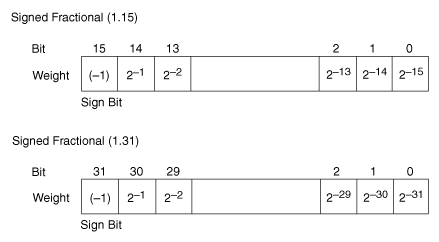
\includegraphics[width=3in]{ang/bf_fract_represent}
\caption{Internal Representation of Fractional Data Types}
\label{bf_fract_represent}
\end{figure}

\begin{table}[H]
\centering
\begin{tabu} to \textwidth {XXXX}
\toprule
Type &Size &Range &Resolution\\
\hline
\texttt{fract16} &16-bit &$-1$ to $1 - 2^{-15}$ &$2^{-15}$\\
\hline
\texttt{fract32} &32-bit &$-1$ to $1 - 2^{-31}$ &$2^{-31}$\\
\bottomrule
\end{tabu}
\caption{Fractional Data Types}
\label{fractional-data-types}
\end{table}

%--------------------------------------------
%--------------------------------------------

\subsection{Performance Tuning Guidelines}

%--------------------------------------------
%--------------------------------------------

\subsection{CrossCore Embedded Studio}

During ELEN90058 \textit{Signal Processing} and ELEN90052 \textit{Advanced Signal Processing} workshop sessions, we used CrossCore\textsuperscript{\textregistered} Embedded Studio to compile and debug code for Blackfin DSP board. Basing on Eclipse, CCES exploits the ecosystem of third-party tools already available to Eclipse developers. Thus, plenty of convenient functions such as plotting arrays of data are available to users \cite{erik-cces}\cite{cces-faq}. CCES could be an ideal substitution for VisualDSP++.\\

However, the AD1980 Audio Codec on ADSP-BF548 EZ-Kit Lite Board is not supported with CCES \cite{cces-ad1980}. Analog Devices engineer Craig Gilchrist explained in \textit{EngineerZone} support community that they do not have a driver for the AD1980 Codec with CCES. In addition, he recommended AD1836 Audio Codec instead \cite{BF548-BSP}.\\

Considering the project budget and potential risk, we eventually decided to stick on VisualDSP++ 5.1.2.

%----------------------------------------------------------------------------------------
%	Section
%----------------------------------------------------------------------------------------

\section{C Program}

\subsection{Audioloopback}

%--------------------------------------------
%--------------------------------------------

\subsection{Pre-emphasis}

It is easy to prove that filter characteristic represented by (\ref{shelving-filter}) will not change if coefficients $a_i$ and $b_i$ are uniformly scaled. Some pre-emphasis filter coefficients (\ref{shleving-coef}) are beyond the fractional data types domain $[-1, 1]$. Hence, the coefficients are scaled by $\lambda$ before converting them from \texttt{float} to \texttt{fract32}.\\

We choose $\lambda = \frac{1}{4}$ primarily because $\frac{1}{a_0} = \frac{1}{\lambda} = 4$ which is a power of 2. In terms of fixed-point data types, left shifting 2 bits is equivalent to multiplying by $\frac{1}{a_0} = 4$ but left shifting is more efficient. Besides, $\lambda = \frac{1}{2}$ is not small enough while $\lambda = \frac{1}{8}$ leads to loss in precision. $a_i \in [-1, 1]$ and $b_i \in [-1, 1]$ for $\forall i = 0, 1, 2$ when $\lambda = \frac{1}{4}$.

\begin{align*}
&\begin{cases}
a_0 = \frac{1}{4} = 0.25\\
a_1 = \frac{-1.523796}{4} = -0.380949\\
a_2 = \frac{0.649345}{4} = 0.162336
\end{cases}
&\begin{cases}
b_0 = \frac{1.861856}{4} = 0.465464\\
b_1 = \frac{-3.102851}{4} = -0.775712\\
b_2 = \frac{1.366544}{4} = 0.341636
\end{cases}
\end{align*}

Filter coefficients are converted into \texttt{fract32} once by \texttt{calc\_shelving\_coef()} function when initializing the system. Finally, all computations in \texttt{pre\_emphasis()} function are fixed-point arithmetic.

%--------------------------------------------
%--------------------------------------------

\subsection{Hamming Window}

For the window length $N = 512$, Hamming window weight $w[n]$ has 512 elements. Table \ref{clocks-hamming} summarizes the efficiency of different methods to obtain $w[n]$. $512/2 = 256$ (due to symmetry) \texttt{fract32} data points occupy 1 KB. There is no reason to recompute them every time. Considering they are most frequently used (180 times per 3-second recording), we store them in the fastest L1 memory. During the initialization session, \texttt{calc\_hamming\_coef} function pre-computes them and converts them into \texttt{frac32}. All computations in \texttt{hamming()} function are fixed-point arithmetic.

\begin{table}[H]
\centering
\begin{tabu} to \textwidth {XXX}
\toprule
Action &clocks &time elapsed\\
\hline
compute &607471 &1.012452 ms\\
\hline
fetch from L1 &8731 &0.014552 ms\\
\hline
fetch from L2 &12827 &0.021378 ms\\
\hline
fetch from external memory &30878 &0.051463 ms\\
\bottomrule
\end{tabu}
\caption{Action Efficiency for Hamming Weights}
\label{clocks-hamming}
\end{table}

From (\ref{eq:windowing}), we have
\begin{equation}
s_j[n] = w[n] s[n+jN] \quad n = 1, 2, \dots, N
\end{equation}
We have known $|s[n+jN]| \le 1$, thus
\begin{equation}
|s_j[n]| = |w[n]| \cdot |s[n+jN]| \le |w[n]| \quad n = 1, 2, \dots, N
\end{equation}
\begin{equation}
\Longrightarrow |s_j[n]|^2 \le |w[n]|^2 \quad n = 1, 2, \dots, N
\end{equation}
\begin{equation}
\Longrightarrow \sum_{n=1}^{N} |s_j[n]|^2 \le \sum_{n=1}^{N} |w[n]|^2
\end{equation}

Based on (\ref{eq:hamming}), for Hamming window length $N = 512$,
\begin{equation}
\sum_{n=1}^{N} |w[n]|^2 = 203.0778 < 256
\end{equation}

Hence,
\begin{equation}
\label{hamming-inequation}
\sum_{n=1}^{N} |s_j[n]|^2 \le \sum_{n=1}^{N} |w[n]|^2 < 256
\end{equation}

%--------------------------------------------
%--------------------------------------------

\subsection{Thresholds}
\subsubsection{Frame Energy}

From (\ref{eq:frame-energy}) and (\ref{hamming-inequation}), we have
\begin{align}
\label{energy-inequation}
&E_s[j] = \sum_{n=1}^{N} |s_j[n]|^2 < 256\\
&\Longrightarrow \sum_{n=1}^{N} \frac{1}{256} |s_j[n]|^2 < 1
\end{align}

(\ref{energy-inequation}) shows that the frame energy will not overflow if we scale the square of amplitudes by $\frac{1}{256}$ before accumulation. Right-shifting the square of amplitudes by $\log_2(256) = 8$ bits is equivalent to multiplying by $\frac{1}{256}$.\\

Right-shifting leads to loss in precision. However, we calculate frame energy only for comparison with the threshold, i.e. the exact value will not be used in further computations, thus the error will not be accumulated. In addition, the change of recording device and environment voice influence much more than the error caused by right-shifting.\\

\texttt{calc\_energy()} function calculates the scaled energy of a frame. Note that the energy threshold (\texttt{ENERGY\_THRESHOLD}) should be scaled by $\frac{1}{256}$ before converted into \texttt{frac32} format during system initialization. Finally, all computations and comparisons related to frame energy are fixed-point arithmetic.
